\section{Initial Assessment}
% got 5,5-6 pages
This initial assessment is the first experiment we performed in the course of this work.
We performed it very early on to get an initial impression on whether our diagnosis of the problem, namely that load balancers are making ineffective decisions and are themselves located too far from clients, is accurate.
We also hoped to get a first impression of how large of a performance uplift might be achievable, and thus whether the performance improvement would justify the additional complexity our approach adds to the system.

The overarching question we want to answer with these experiments is whether more complex load balancing, such as least response time load balancing, and moving the load balancers closer to the clients leads to overall performance improvements.
We also want to understand what impact on performance we could expect from implementing only one of the two proposed improvements.

\subsubsection{Setup}
To answer these questions we test four load balancer configurations in three different scenarios.
\paragraph{Load Balancer Setup}
To assess the role of the load balancer implementation, we compare typical round robin load balancing, as it is found in current serverless frameworks such as OpenFaaS\cite{openfaas} and their underlying container orchestration service\cite{kubernetes}, and least response time load balancing to represent more sophisticated load balancing decisions.

Since this experiment is performed before the others we rely on an initial parametrization and implementation, which differs slightly from the one we ultimately propose.
The weight range is [1;10], with a scaling factor of 1, and a weight update interval of 15 seconds.
Furthermore we rely on a different implementation of weighted round robin\cite{wrr-kblinux}, which is functionally very similar but works through upstreams iteratively by their weight, instead of the more intermixed upstream selection we describe in our approach.
In this implementation, there is also a notion of current weights\cite{wrr-kblinux}, and they are reset every time the weights are updated.
\paragraph{Load balancer scaling and placement}
For the load balancer location we evaluate the two most extreme scenarios: A single centralized load balancing instance which serves all client requests, and a maximally distributed scenario in which every single node in the system also hosts a load balancer instance.

This gives us four load balancer configurations:
\begin{itemize}
    \item Round Robin centralized
    \item Round Robin on all nodes
    \item Least Response Time centralized
    \item Least response time on all nodes
\end{itemize}

Each of these four configurations is evaluated in three different scenarios, which represent clusters of different size and network topology.
These topologies are oriented on a smart city/urban sensing type application.
\begin{itemize}
    \item City
    \item Nation
    \item Global
\end{itemize}
\paragraph{City}
In this scenario the cluster is set to a size of 100 nodes, which are assumed to all be located in the same city, meaning network latencies between nodes are small.
The city features a data center which consists of about 50\% of the total node count, and features nodes with high compute capability, partially with GPU acceleration.
The rest of the nodes are assumed to be distributed across the city closer to clients, and consist to two thirds of medium performance nodes, and one third low performance nodes.
\paragraph{Nation}
This scenario features a larger cluster that spans over three cities.
Each of those cities features the same relative node distribution as the previous scenario.
We chose the USA as our example, as using a small country such as Austria would not provide significant enough latency differences between cities.
Our scenario features the cities of Chicago with 100 nodes, Seattle with 100 nodes, and New York with 150 nodes.
While nodes within the same city feature extremely low network latency, nodes across two cities have more significant network distances between them.

 \begin{table}[]
\centering
\begin{tabular}{r|ccc}
\multicolumn{1}{c|}{} & \textbf{Chicago} & \textbf{New York} & \textbf{Seattle} \\ \hline
\textbf{Chicago}      & -                & 31ms              & 55ms             \\
\textbf{New York}     & 31ms             & -                 & 75ms             \\
\textbf{Seatte}       & 55ms             & 75ms              & -                \\ \hline
\end{tabular}
\caption{Network latencies between cities in the initial \textbf{nation} evaluation scenario. Latencies are taken from Wonder Network's global ping statistics\cite{wondernetworkGlobalPingStatistics}}
\label{tab:initial_nation_pings}
\end{table}

\begin{table}[]
\centering
\begin{tabular}{r|ccc}
\multicolumn{1}{c|}{} & \textbf{New York} & \textbf{London} & \textbf{Sydney} \\ \hline
\textbf{New York}     & -                 & 86ms            & 204ms           \\
\textbf{London}       & 86ms              & -               & 253ms           \\
\textbf{Sydney}       & 204ms             & 253ms           & -               \\ \hline
\end{tabular}

\caption{Network latencies between cities in the initial \textbf{global} evaluation scenario. Latencies are taken from Wonder Network's global ping statistics\cite{wondernetworkGlobalPingStatistics}}
\label{tab:initial_global_pings}
\end{table}   

The network latencies between the cities are taken from Wonder Network\cite{wondernetworkGlobalPingStatistics}, and can be seen in Table \ref{tab:initial_nation_pings}

\paragraph{Global}
The global scenario once again features three cities, but they are distributed not just within a single country, but across the globe.
The cities are New York with 100 nodes, London with 100 nodes, and Sydney with 150 nodes.
Network latencies can be seen in Table \ref{tab:initial_global_pings}.

\paragraph{Clients}
Each scenarios features a client ratio of 0.6, meaning there are 60\% as many clients as there are compute nodes.
Clients are assumed to be on the edge of the network and thus closest to the medium and small sized compute nodes.

\paragraph{Functions and request load}
We use our basic three function deployments for these experiments.
To isolate the system behaviour on the effect of load balancer implementation, scale and placement we disabled the normal function scaling behaviour.
Instead the system immediately sets a fixed scale for each function such that on each node in the entire cluster a function replica is started.
We consider the functions to be of equal importance, thus each function starts up $\frac{n}{3}$ replicas where $n$ is the total number of nodes.
Lastly all experiments simulate a timeframe of 1000 seconds, and feature a request load of 75\gls{rps}.

\subsubsection{Results}

\begin{table}[]
\begin{tabular}{lrrrr}
\hline
                                 & \multicolumn{4}{c}{mean}                                                                                                                              \\
\textbf{Load Balancer Type}      & \multicolumn{1}{r}{\textbf{TRT}} & \multicolumn{1}{r}{\textbf{FET}} & \multicolumn{1}{r}{\textbf{Net CL-LB}} & \multicolumn{1}{r}{\textbf{Net LB-FX}} \\ \hline
\multicolumn{5}{c}{City Scale Evaluation}                                                                                                                                                \\ \hline
Round Robin centralized          & 0.0\%                            & 0.0\%                            & 0.0\%                                  & 0.0\%                                  \\
Round Robin on all nodes         & 13.3\%                           & 0.0\%                            & 35.4\%                                 & 30.3\%                                 \\
Least Response Time centralized  & 32.7\%                           & 47.9\%                           & 15.8\%                                 & 24.6\%                                 \\
Least Response Time on all nodes & 81.3\%                           & 109.3\%                          & 51.6\%                                 & 61.9\%                                 \\ \hline
\multicolumn{5}{c}{Nation Scale Evaluation}                                                                                                                                              \\ \hline
Round Robin centralized          & 0.0\%                            & 0.0\%                            & 0.0\%                                  & 0.0\%                                  \\
Round Robin on all nodes         & 95.7\%                           & -0.4\%                           & 1028.2\%                               & 34.8\%                                 \\
Least Response Time centralized  & 18.1\%                           & 27.8\%                           & 3.0\%                                  & 34.7\%                                 \\
Least Response Time on all nodes & 312.0\%                          & 86.9\%                           & 1065.6\%                               & 257.5\%                                \\ \hline
\multicolumn{5}{c}{Global Scale Evaluation}                                                                                                                                              \\ \hline
Round Robin centralized          & 0.0\%                            & 0.0\%                            & 0.0\%                                  & 0.0\%                                  \\
Round Robin on all nodes         & 82.8\%                           & -0.7\%                           & 2910.6\%                               & -5.3\%                                 \\
Least Response Time centralized  & 21.0\%                           & 18.4\%                           & 0.0\%                                  & 60.8\%                                 \\
Least Response Time on all nodes & 606.9\%                          & 77.3\%                           & 2997.8\%                               & 428.2\%                                \\ \hline
\end{tabular}
\caption{ Percentage improvement in mean values of a single experimental run of the initial evaluation in different scenarios. Displayed mean values are in order: \gls{trt}, \gls{fet}, network time between client and load balancer, and network time between load balancer and function replica}
\label{tab:initial_eval_results_mean}
\end{table}

\begin{table}[]
\begin{tabular}{lrrrr}
\hline
                                 & \multicolumn{4}{c}{50th percentile (median)}                                                                                                          \\
\textbf{Load Balancer Type}      & \multicolumn{1}{r}{\textbf{TRT}} & \multicolumn{1}{r}{\textbf{FET}} & \multicolumn{1}{r}{\textbf{Net CL-LB}} & \multicolumn{1}{r}{\textbf{Net LB-FX}} \\ \hline
\multicolumn{5}{c}{City Scale Evaluation}                                                                                                                                                \\ \hline
Round Robin centralized          & 0.0\%                            & 0.0\%                            & 0.0\%                                  & 0.0\%                                  \\
Round Robin on all nodes         & 26.5\%                           & 0.0\%                            & 34.0\%                                 & 25.1\%                                 \\
Least Response Time centralized  & 34.8\%                           & 183.0\%                          & 5.0\%                                  & 13.5\%                                 \\
Least Response Time on all nodes & 93.3\%                           & 185.6\%                          & 37.0\%                                 & 37.7\%                                 \\ \hline
\multicolumn{5}{c}{Nation Scale Evaluation}                                                                                                                                              \\ \hline
Round Robin centralized          & 0.0\%                            & 0.0\%                            & 0.0\%                                  & 0.0\%                                  \\
Round Robin on all nodes         & 109.0\%                          & -7.9\%                           & 1674.1\%                               & 76.2\%                                 \\
Least Response Time centralized  & 23.5\%                           & 16.1\%                           & 4.3\%                                  & 118.2\%                                \\
Least Response Time on all nodes & 350.4\%                          & 22.9\%                           & 1674.1\%                               & 1316.4\%                               \\ \hline
\multicolumn{5}{c}{Global Scale Evaluation}                                                                                                                                              \\ \hline
Round Robin centralized          & 0.0\%                            & 0.0\%                            & 0.0\%                                  & 0.0\%                                  \\
Round Robin on all nodes         & 27.6\%                           & 0.0\%                            & 5338.8\%                               & 95.0\%                                 \\
Least Response Time centralized  & 9.8\%                            & 0.6\%                            & 0.0\%                                  & 1498.5\%                               \\
Least Response Time on all nodes & 1653.3\%                         & 25.9\%                           & 5338.8\%                               & 4541.5\%                               \\ \hline
\end{tabular}
\caption{50th percentile (i.e. median) values of a single experimental run of the initial evaluation in different scenarios. Displayed values are in order: \gls{trt}, \gls{fet}, network time between client and load balancer, and network time between load balancer and function replica}
\label{tab:initial_eval_results_q50}
\end{table}

\begin{figure}
    \centering
    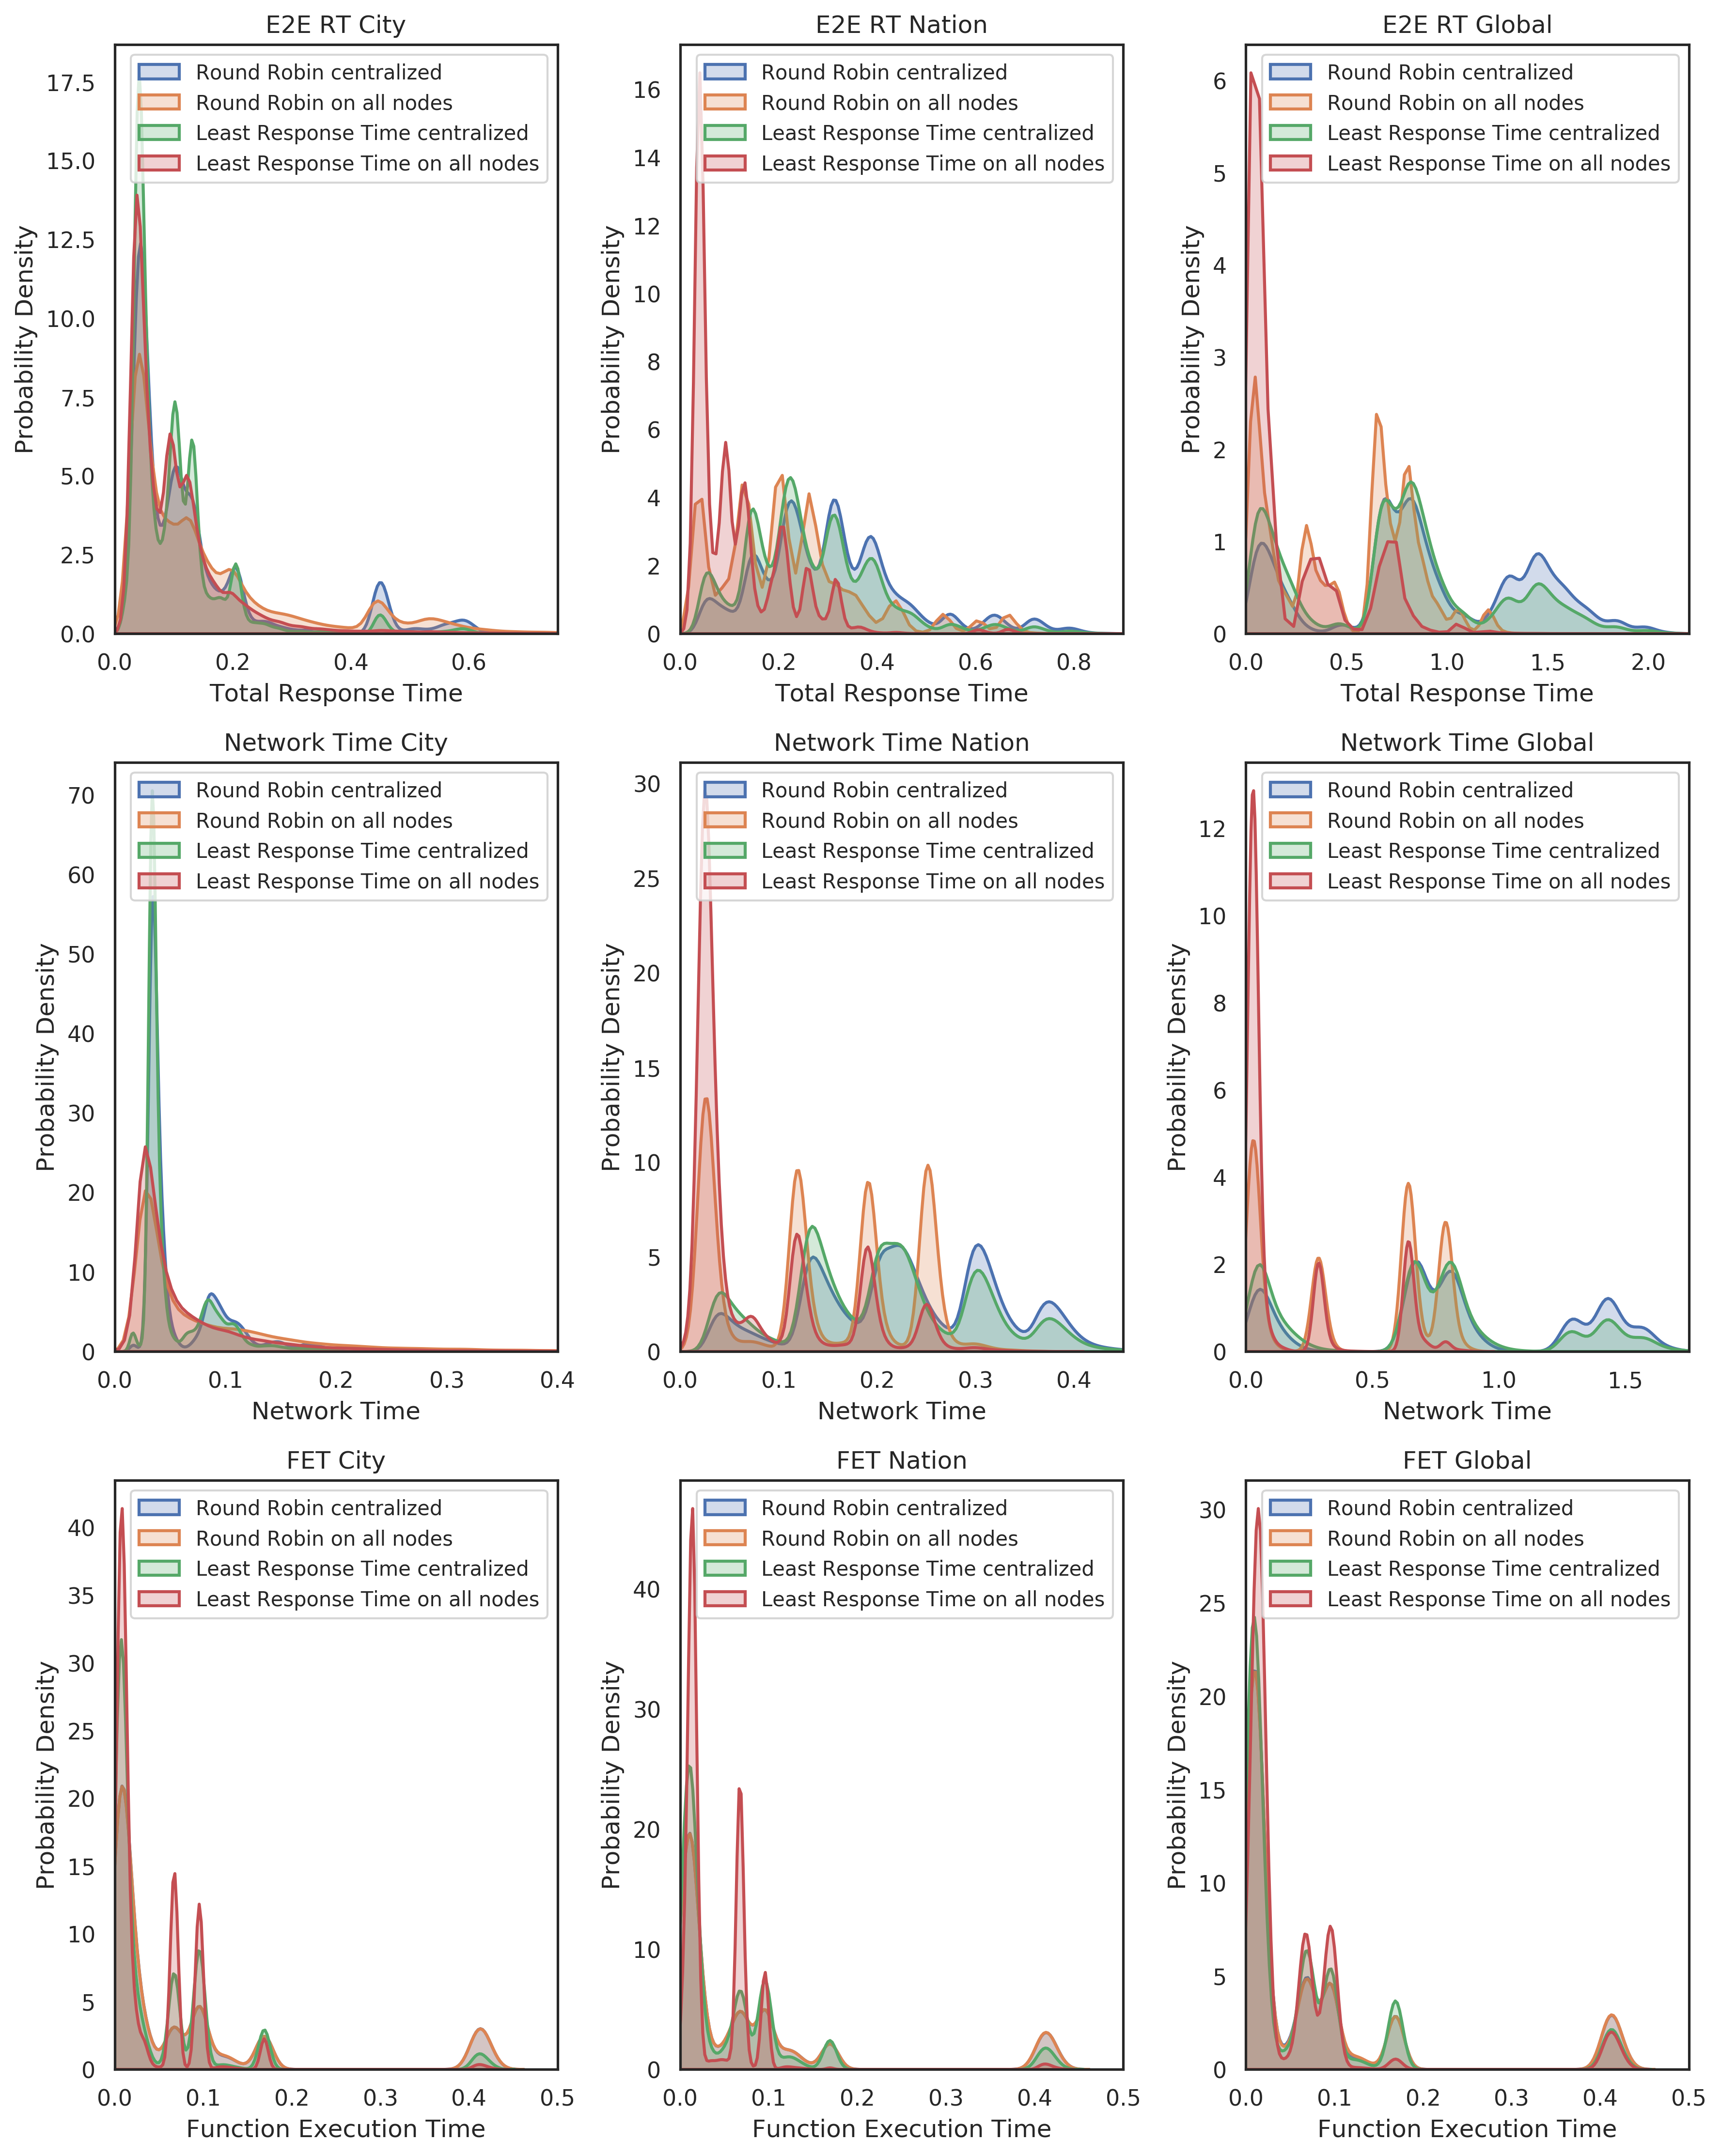
\includegraphics[width=\linewidth]{graphics/graphs/initial_eval_pdfs_3x3_hires.png}
    \caption{Kernel Density Estimate of a single experiment run. Shown data can be interpreted as probability density functions. Data is visualized for \gls{trt}, \gls{fet} and the time incurred through network transfers.}
    \label{fig:initial_eval_pdfs}
\end{figure}

Since the experiments feature a significant degree of random sampling in their simulation as function location, \gls{fet} sampling and client positions are random, we ran each experiment 10 times.
The results presented here are those of a single experimental run, since no runs showed significantly different results.
Table \ref{tab:initial_eval_results_mean} shows the percentage improvement different load balancer types and scales give when compared to the default centralized round robin.
Here the mean values of the \gls{trt}, \gls{fet}, and network times between client and load balancer, and load balancer and function replica are shown.
Both a more sophisticated approach to load balancing and moving load balancer instances closer to the clients shows significant performance improvements, but across the board only the combination of these two improvements (i.e. least response time on all nodes) gives the most significant performance uplift.
We can also see that least response time load balancing not only improves network times between the load balancer and the function replica, but also decreases \gls{fet}.
In addition we observe that the performance improvement given through distributed least response time load balancing becomes larger in geographically more distributed scenarios.

Table \ref{tab:initial_eval_results_q50} shows the difference between the median of these metrics.
Here the performance uplift achieved by least response time load balancing on all nodes become even larger, up to a 16,5x improvement in \gls{trt} in the global scenario.

For even more detailed analyses figure \ref{fig:initial_eval_pdfs} shows the probability density function estimated of the same experimental run.
Note that \textit{E2E RT} in this figure means \gls{trt}.
Here the overall trend observed in the tables \ref{tab:initial_eval_results_mean} and \ref{tab:initial_eval_results_q50} carries through, showing that least response time on all nodes not only improves average performance, but pushes the whole distribution towards faster \gls{fet} and lower network times.